
\chapter{2. Linear PDEs: structured grids}

We start with the Poisson problem because it is the right place to start.  Though it is a cliche in applied mathematics, in solving it we will use key parts of \PETSc: build a structured grid using a \PETSc \pDMDA, assemble a \pMat and some \pVecs in parallel on this grid, and solve in parallel using a \pKSP object.

\section{A Poisson problem on a square}

The \emph{Laplacian} is the most common second-derivative of a function $u(x,y)$ in the plane:
    $$\grad^2 u = \Div(\grad u) = \frac{\partial^2 u}{\partial x^2} + \frac{\partial^2 u}{\partial y^2}.$$
When one sees it in a mathematical model, the Laplacian almost always appears because of the conservation of the quantity $u$ (thus the divergence $\Div$) and an assumption that the gradient $\grad u$ is, up to a coefficient, the flux of $u$ \citep{Ockendonetal2003}.  

In the \emph{Poisson equation} the Laplacian of $u$ is equal to a known function.  We will not just solve this one equation, however, but a \emph{Poisson problem}, on a finite region and including boundary conditions, which together determine a unique solution \citep{Evans}.  Let $\mathcal{S}$ be the open unit square $(0,1)\times(0,1)$ in the plane.  The following is our first Poisson problem, as shown in Figure \ref{fig:unitsquare}:
\begin{marginfigure}
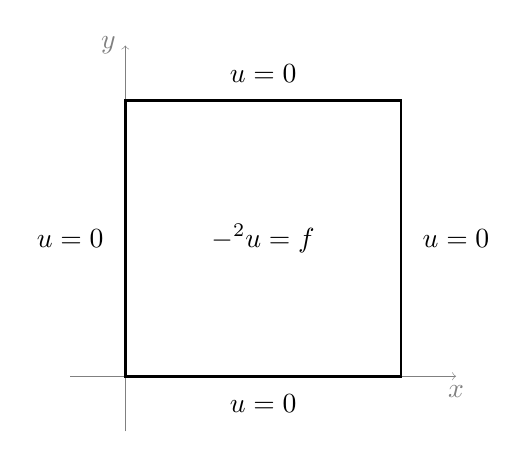
\begin{tikzpicture}[scale=3.5]
  \draw[->,gray,very thin] (-0.2,0.0) -- (1.2,0.0) node[below] {$x$};
  \draw[->,gray,very thin] (0.0,-0.2) -- (0.0,1.2) node[left] {$y$};
  \draw[line width=1.0pt] (0.0,0.0) -- (0.0,1.0) -- (1.0,1.0) -- (1.0,0.0) -- cycle;
  \node at (0.5,0.5) {$- \grad^2 u = f$};
  \node at (0.5,-0.1) {$u = 0$};
  \node at (0.5,1.1) {$u = 0$};
  \node at (-0.2,0.5) {$u = 0$};
  \node at (1.2,0.5) {$u = 0$};
\end{tikzpicture}
\caption{Our first, simple goal is to solve the Poisson equation on the unit square $\mathcal{S}$, with homogeneous Dirichlet boundary conditions.}
\label{fig:unitsquare}
\end{marginfigure}
\begin{align}
- \grad^2 u &= f \quad \text{ on } \mathcal{S}, \label{poissonsquare} \\
u &= 0 \quad \text{ on } \partial \mathcal{S}. \notag
\end{align}
The boundary of the unit square, denoted ``$\partial\mathcal{S}$'', is simply union of four (closed) line segments.  The boundary conditions $u=0$ are called ``\emph{homogeneous Dirichlet}.''

The Poisson problem models the distribution of temperature in a conducting object at steady state, the electrostatic potential, the equilibrium distribution from certain random walks, and many other other physical phenomena.  For example, we can illustrate the above comment about the appearance of the Laplacian in the context of heat conduction.  In that case the heat flux is $\bq = - \grad u$ (up to a multiplied constant) if $u$ is the temperature, while the steady-state conservation of heat energy balances the divergence of the flux with the heat source $f$, that is $\Div \bq = f$, again up to a multiplied constant.  This is the Poisson equation \eqref{poissonsquare}.  Holding the temperature fixed at zero along the boundary completes the problem.

Without any boundary conditions, the Poisson equation $-\grad^2 u = f$ alone is not a well-posed problem because if $-\grad^2 u = f$ then also $-\grad^2(u+C)=f$ for any constant $C$; there are many solutions.  With Dirichlet boundary conditions, the solution is at least unique; see Theorem 5 in section 2.2 of \citet{Evans} or subsection 5.2.1 of \citet{Ockendonetal2003}.

For this chapter we will suppose $f(x,y)$ is continuous and bounded on $\mathcal{S}$, so that we can compute its pointwise values.  With our homogeneous Dirichlet boundary conditions, and the assumptions on $f$, standard theory\sidenote{One approach to showing this classical-existence fact solves the problem \eqref{poissonsquare} by Fourier series!  Because $f$ itself is square-integrable, the Fourier coefficients $\hat f$ are square-integrable (Parseval's equality).  Because the Laplacian is elliptic and second-order, the coefficients $\hat u$ are square-integrable even when multiplied by the square of the frequency.  By a Cauchy-Schwarz argument, one then shows that the Fourier series for $u$ is a sequence of continuous functions on $\overline{\mathcal{S}}$ which converge uniformly.  (\emph{For a more abstract version see Theorem 6 in section 5.6 of \citet{Evans}, namely a general Sobolev inequality, in the case of the plane ($n=2$), square-integrable functions ($p=2$) and two derivatives ($k=2$).})} says that $u(x,y)$ exists and is continuous on the closed square $\overline{\mathcal{S}}$.  Thus there is no ambiguity in the boundary condition ``$u=0$ on $\partial \mathcal{S}$,'' and furthermore we can sensibly discuss the pointwise values $u(x,y)$.


\section{A finite difference method}

Because \eqref{poissonsquare} is a linear problem, finite-dimensional approximations of it are simply linear systems.  Such a finite-dimensional approximation comes from applying a \emph{finite difference} (FD) method.

To start our FD method we put a \emph{structured grid} of $MN$ points on the unit square, as in Figure \ref{fig:unitsquaregrid}, with spacing $h_x=1/(M-1)$ and $h_y=1/(N-1)$ in the two directions.  Thus the grid locations are $x_i = i\, h_x$ and $y_j = j\, h_y$ for $i = 0,1,\dots,M-1$ and $j=0,1,\dots,N-1$.

\begin{marginfigure}
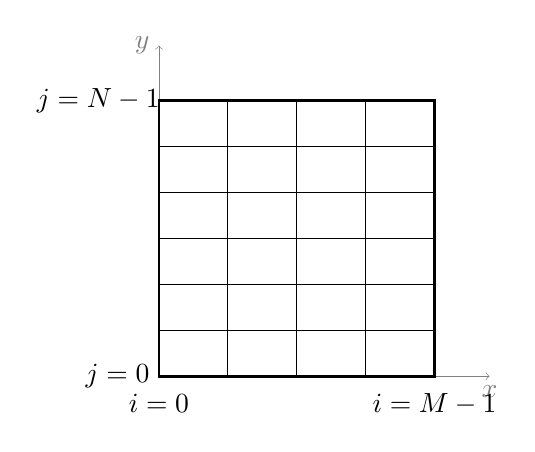
\begin{tikzpicture}[scale=3.5]
  \draw[->,gray,very thin] (0.0,0.0) -- (1.2,0.0) node[below] {$x$};
  \draw[->,gray,very thin] (0.0,0.0) -- (0.0,1.2) node[left] {$y$};
  \draw[line width=1.0pt] (0.0,0.0) -- (0.0,1.0) -- (1.0,1.0) -- (1.0,0.0) -- cycle;
  \node at (0.0,-0.1) {$i=0$};
  \node at (1.0,-0.1) {$i=M-1$};
  \node at (-0.15,0.0) {$j=0$};
  \node at (-0.22,1.0) {$j=N-1$};
  \draw[xstep=0.25,ystep=0.166667,black,thin] (0.0,0.0) grid (1.0,1.0);
\end{tikzpicture}
\caption{A grid on the unit square $\mathcal{S}$, with $M=5$ and $N=7$.}
\label{fig:unitsquaregrid}
\end{marginfigure}

The construction of such a two-dimensional (2D) grid, and the distribution of it across processors, is our first new idea from \PETSc after the \pVec and \pMat basics in Chapter 1.  We will create a \PETSc \pDM object.\sidenote{``\pDM'' might stand for ``data management'', but perhaps ``distributed mesh'' is a better expansion.  You choose.}  A \pDM is an abstract type for describing the topology (i.e.~connectedness) of a grid, and the way it is distributed across \MPI processes.  Consider these lines:
\begin{Verbatim}[fontsize=\small]
  DM  da;
  DMDACreate2d(PETSC_COMM_WORLD,
               DM_BOUNDARY_NONE, DM_BOUNDARY_NONE, DMDA_STENCIL_STAR,
               -9,-9,PETSC_DECIDE,PETSC_DECIDE,1,1,NULL,NULL,
               &da);
  DMDASetUniformCoordinates(da,0.0,1.0,0.0,1.0,-1.0,-1.0);
\end{Verbatim}
\medskip\noindent
Note \texttt{da} is created to have type ``\pDMDA'', which is the subclass of \pDM s which are structured grids.  The command \texttt{DMDACreate2d()} creates this object as a 2D structured grid with default dimensions $M=9$ and $N=9$; these defaults are set using negative numbers as arguments, and then will be overridden at runtime by options \texttt{-da\_grid\_x} and \texttt{-da\_grid\_y}.  (The several other arguments to \texttt{DMDACreate2d()} will be addressed in a moment.)  The call to \texttt{DMDASetUniformCoordinates()} sets the domain to be $[0,1]\times[0,1]$; the last two arguments are ignored in this case but would set limits on the third dimension in 3D.


On the other hand, by a well-known Taylor's theorem argument \citep{MortonMayers}, for any function $F(x)$ which is sufficiently smooth,
    $$F''(x) = \frac{F(x+h) - 2 F(x) + F(x-h)}{h^2} + O(h^2)$$
as $h$ goes to zero.  To apply this formula to approximating the Laplacian in problem \eqref{poissonsquare}, we let $U_{i,j}$ be the approximation (which we compute) to the exact value $u(x_i,y_j)$ (which we don't suppose to know) of the solution $u$.  Also we denote $f_{i,j} = f(x_i,y_j)$.  Then we have this FD approximation to problem \eqref{poissonsquare}:
\begin{equation}
- \frac{U_{i+1,j} - 2 U_{i,j} + U_{i-1,j}}{h_x^2} - \frac{U_{i,j+1} - 2 U_{i,j} + U_{i,j-1}}{h_y^2} = f_{i,j}. \label{poissonsquareFD}
\end{equation}
Equation \eqref{poissonsquareFD} applies for all of the interior points where $1 \le i \le M-2$ and $1 \le j \le N-2$.  The boundary conditions in \eqref{poissonsquare} become $U_{0,j} = U_{M-1,j} = U_{i,0} = U_{i,N-1} = 0$, for all $i,j$.

Problem \eqref{poissonsquareFD} is a linear system.  We choose to treat all $MN$ locations on the grid as unknowns. FIXME: BUILD MATRIX, COMMENTING ON ROW SCALING (i.e. mult by $h_x h_y$ to improve conditioning)


\begin{marginfigure}
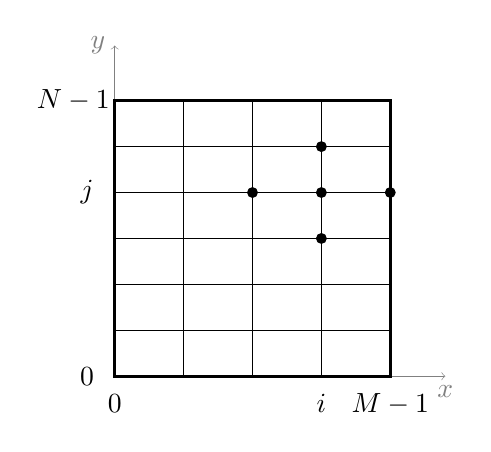
\begin{tikzpicture}[scale=3.5]
  \draw[->,gray,very thin] (0.0,0.0) -- (1.2,0.0) node[below] {$x$};
  \draw[->,gray,very thin] (0.0,0.0) -- (0.0,1.2) node[left] {$y$};
  \draw[line width=1.0pt] (0.0,0.0) -- (0.0,1.0) -- (1.0,1.0) -- (1.0,0.0) -- cycle;
  \node at (0.0,-0.1) {$0$};
  \node at (0.75,-0.1) {$i$};
  \node at (1.0,-0.1) {$M-1$};
  \node at (-0.1,0.0) {$0$};
  \node at (-0.1,0.666667) {$j$};
  \node at (-0.15,1.0) {$N-1$};
  \filldraw (0.50,0.666667) circle (0.5pt);
  \filldraw (0.75,0.666667) circle (0.5pt);
  \filldraw (1.00,0.666667) circle (0.5pt);
  \filldraw (0.75,0.5) circle (0.5pt);
  \filldraw (0.75,0.833333) circle (0.5pt);
  \draw[xstep=0.25,ystep=0.166667,black,thin] (0.0,0.0) grid (1.0,1.0);
\end{tikzpicture}
\caption{A stencil is shown on the grid at $i=3$ and $j=4$.}
\label{fig:unitsquaregridstencil}
\end{marginfigure}

\cinput{structuredlaplacian.c}{Fill matrix entries using \texttt{MatSetValuesStencil}.}{//CREATEMATRIX}{//ENDCREATEMATRIX}{code:structuredlaplacian}

\cinputpart{c2poisson.c}{The right side of equation \eqref{poissongridsystem} comes from differentiating the exact solution, which this method also computes.}{I}{//RHS}{//ENDRHS}{code:ctwopoissonrhs}

\cinputpart{c2poisson.c}{Set up \pDMDA \texttt{da} and \pMat \texttt{A} objects, and assemble the latter by calling \texttt{formlaplacian()}.}{II}{//CREATE}{//ENDCREATE}{code:ctwopoissoncreate}

\cinputpart{c2poisson.c}{Solve using \pKSP, and report on solution.}{III}{//SOLVE}{//ENDSOLVE}{code:ctwopoissonsolve}

\section{Runtime control of linear solver}

FIXME: basic Krylov theory

\section{Time-dependent heat equation}

FIXME: we WON'T do explicit, but it would look like ...

FIXME: use TS for backward-euler
